% Options for packages loaded elsewhere
\PassOptionsToPackage{unicode}{hyperref}
\PassOptionsToPackage{hyphens}{url}
%
\documentclass[
  ignorenonframetext,
]{beamer}
\usepackage{pgfpages}
\setbeamertemplate{caption}[numbered]
\setbeamertemplate{caption label separator}{: }
\setbeamercolor{caption name}{fg=normal text.fg}
\beamertemplatenavigationsymbolsempty
% Prevent slide breaks in the middle of a paragraph
\widowpenalties 1 10000
\raggedbottom
\setbeamertemplate{part page}{
  \centering
  \begin{beamercolorbox}[sep=16pt,center]{part title}
    \usebeamerfont{part title}\insertpart\par
  \end{beamercolorbox}
}
\setbeamertemplate{section page}{
  \centering
  \begin{beamercolorbox}[sep=12pt,center]{part title}
    \usebeamerfont{section title}\insertsection\par
  \end{beamercolorbox}
}
\setbeamertemplate{subsection page}{
  \centering
  \begin{beamercolorbox}[sep=8pt,center]{part title}
    \usebeamerfont{subsection title}\insertsubsection\par
  \end{beamercolorbox}
}
\AtBeginPart{
  \frame{\partpage}
}
\AtBeginSection{
  \ifbibliography
  \else
    \frame{\sectionpage}
  \fi
}
\AtBeginSubsection{
  \frame{\subsectionpage}
}
\usepackage{amsmath,amssymb}
\usepackage{lmodern}
\usepackage{ifxetex,ifluatex}
\ifnum 0\ifxetex 1\fi\ifluatex 1\fi=0 % if pdftex
  \usepackage[T1]{fontenc}
  \usepackage[utf8]{inputenc}
  \usepackage{textcomp} % provide euro and other symbols
\else % if luatex or xetex
  \usepackage{unicode-math}
  \defaultfontfeatures{Scale=MatchLowercase}
  \defaultfontfeatures[\rmfamily]{Ligatures=TeX,Scale=1}
  \setmainfont[BoldFont = SF Pro Rounded Semibold]{SF Pro Rounded}
  \setmathfont[]{STIX Two Math}
\fi
\usefonttheme{serif} % use mainfont rather than sansfont for slide text
% Use upquote if available, for straight quotes in verbatim environments
\IfFileExists{upquote.sty}{\usepackage{upquote}}{}
\IfFileExists{microtype.sty}{% use microtype if available
  \usepackage[]{microtype}
  \UseMicrotypeSet[protrusion]{basicmath} % disable protrusion for tt fonts
}{}
\makeatletter
\@ifundefined{KOMAClassName}{% if non-KOMA class
  \IfFileExists{parskip.sty}{%
    \usepackage{parskip}
  }{% else
    \setlength{\parindent}{0pt}
    \setlength{\parskip}{6pt plus 2pt minus 1pt}}
}{% if KOMA class
  \KOMAoptions{parskip=half}}
\makeatother
\usepackage{xcolor}
\IfFileExists{xurl.sty}{\usepackage{xurl}}{} % add URL line breaks if available
\IfFileExists{bookmark.sty}{\usepackage{bookmark}}{\usepackage{hyperref}}
\hypersetup{
  pdftitle={444 Lecture 2.9 - Nash Equilibrium},
  pdfauthor={Brian Weatherson},
  hidelinks,
  pdfcreator={LaTeX via pandoc}}
\urlstyle{same} % disable monospaced font for URLs
\newif\ifbibliography
\usepackage{graphicx}
\makeatletter
\def\maxwidth{\ifdim\Gin@nat@width>\linewidth\linewidth\else\Gin@nat@width\fi}
\def\maxheight{\ifdim\Gin@nat@height>\textheight\textheight\else\Gin@nat@height\fi}
\makeatother
% Scale images if necessary, so that they will not overflow the page
% margins by default, and it is still possible to overwrite the defaults
% using explicit options in \includegraphics[width, height, ...]{}
\setkeys{Gin}{width=\maxwidth,height=\maxheight,keepaspectratio}
% Set default figure placement to htbp
\makeatletter
\def\fps@figure{htbp}
\makeatother
\setlength{\emergencystretch}{3em} % prevent overfull lines
\providecommand{\tightlist}{%
  \setlength{\itemsep}{0pt}\setlength{\parskip}{0pt}}
\setcounter{secnumdepth}{-\maxdimen} % remove section numbering
\let\Tiny=\tiny

 \setbeamertemplate{navigation symbols}{} 

% \usetheme{Madrid}
 \usetheme[numbering=none, progressbar=foot]{metropolis}
 \usecolortheme{wolverine}
 \usepackage{color}
 \usepackage{MnSymbol}
% \usepackage{movie15}

\usepackage{amssymb}% http://ctan.org/pkg/amssymb
\usepackage{pifont}% http://ctan.org/pkg/pifont
\newcommand{\cmark}{\ding{51}}%
\newcommand{\xmark}{\ding{55}}%

\DeclareSymbolFont{symbolsC}{U}{txsyc}{m}{n}
\DeclareMathSymbol{\boxright}{\mathrel}{symbolsC}{128}
\DeclareMathAlphabet{\mathpzc}{OT1}{pzc}{m}{it}

\setlength{\parskip}{1ex plus 0.5ex minus 0.2ex}

\AtBeginSection[]
{
\begin{frame}
	\Huge{\color{darkblue} \insertsection}
\end{frame}
}

\renewenvironment*{quote}	
	{\list{}{\rightmargin   \leftmargin} \item } 	
	{\endlist }

\definecolor{darkgreen}{rgb}{0,0.7,0}
\definecolor{darkblue}{rgb}{0,0,0.8}

\usepackage[italic]{mathastext}
\usepackage{nicefrac}


%\def\toprule{}
%\def\bottomrule{}
%\def\midrule{}
\usepackage{etoolbox}
\AfterEndEnvironment{description}{\vspace{9pt}}
\AfterEndEnvironment{oltableau}{\vspace{9pt}}
\BeforeBeginEnvironment{oltableau}{\vspace{9pt}}
\AfterEndEnvironment{center}{\vspace{9pt}}
\BeforeBeginEnvironment{tabular}{\vspace{9pt}}
\AfterEndEnvironment{longtable}{\vspace{-6pt}}
\usepackage{booktabs}
\usepackage{longtable}
\usepackage{array}
\usepackage{multirow}
\usepackage{wrapfig}
\usepackage{float}
\usepackage{colortbl}
\usepackage{pdflscape}
\usepackage{tabu}
\usepackage{threeparttable} 
\usepackage{threeparttablex} 
\usepackage[normalem]{ulem} 
\usepackage{makecell}
\usepackage{xcolor}
\usepackage{ulem}

\setlength\heavyrulewidth{0ex}
\setlength\lightrulewidth{0.08ex}

\aboverulesep=0ex
\belowrulesep=0ex
\renewcommand{\arraystretch}{1.2}
\ifluatex
  \usepackage{selnolig}  % disable illegal ligatures
\fi

\title{444 Lecture 2.9 - Nash Equilibrium}
\author{Brian Weatherson}
\date{}

\begin{document}
\frame{\titlepage}

\begin{frame}{Plan}
\protect\hypertarget{plan}{}
To introduce the most famous concept in game theory, Nash Equilibrium.
\end{frame}

\begin{frame}{Reading}
\protect\hypertarget{reading}{}
Bonanno, section 2.6.
\end{frame}

\begin{frame}{John Nash}
\protect\hypertarget{john-nash}{}
\begin{columns}[c]
\begin{column}{0.48\textwidth}
\begin{figure}
\centering
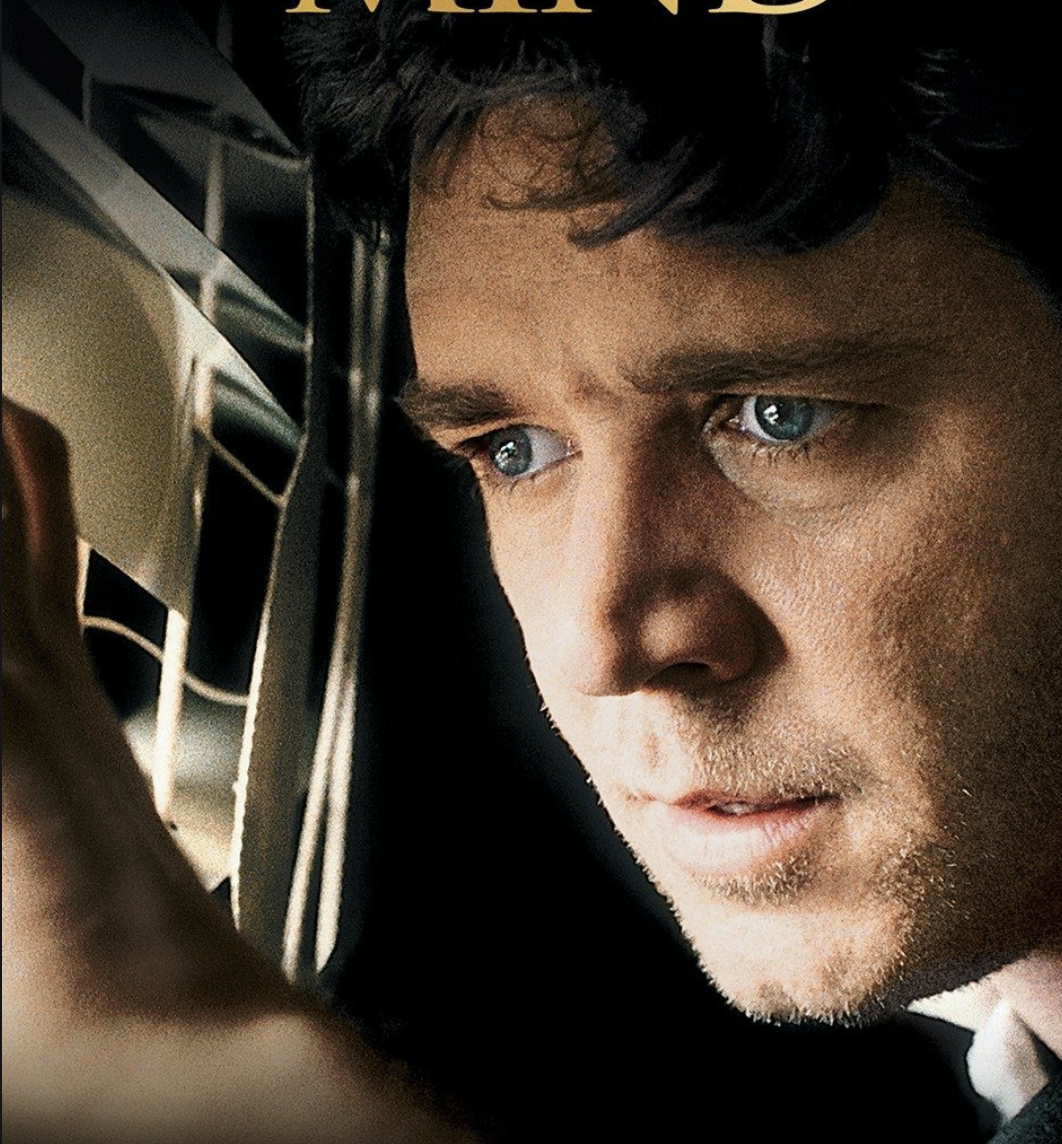
\includegraphics[width=0.75\textwidth,height=0.75\textheight]{images/crowe.png}
\caption{John Nash (via Hollywood)}
\end{figure}
\end{column}

\begin{column}{0.48\textwidth}
\begin{itemize}
\tightlist
\item
  Nash Equilibrium is named after the American mathematician John Nash.
\item
  Except I seem to have a picture of Russell Crowe here.
\end{itemize}
\end{column}
\end{columns}
\end{frame}

\begin{frame}{John Nash}
\protect\hypertarget{john-nash-1}{}
\begin{columns}[c]
\begin{column}{0.48\textwidth}
\begin{figure}
\centering
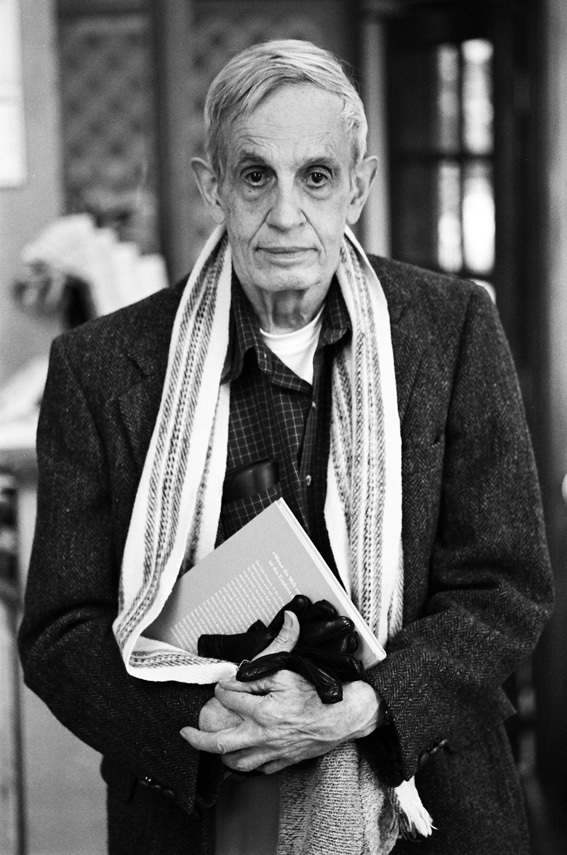
\includegraphics[width=0.75\textwidth,height=0.75\textheight]{images/nash.jpg}
\caption{John Nash}
\end{figure}
\end{column}

\begin{column}{0.48\textwidth}
\begin{itemize}
\tightlist
\item
  Nash Equilibrium is named after the American mathematician John Nash
  (1928-2015).
\item
  It is the core concept of contemporary game theory.
\end{itemize}
\end{column}
\end{columns}
\end{frame}

\begin{frame}{Best Response}
\protect\hypertarget{best-response}{}
\begin{itemize}
\tightlist
\item
  We will build up to it in stages.
\item
  The first important notion is that of a best response.
\item
  Strategy \(S\) is a best response to strategies by the other players
  iff no other strategy can do better, given what the other players are
  doing.
\end{itemize}
\end{frame}

\begin{frame}{Example}
\protect\hypertarget{example}{}
\begin{table}[!h]
\centering
\begin{tabular}[t]{>{}r|ccc}
\toprule
 & Left & Center & Right\\
\midrule
Up & 4, 3 & 2, 0 & 0, 5\\
Middle & 6, 2 & 0, 4 & 3, 1\\
Down & 3, 0 & 2, 1 & 4, 2\\
\bottomrule
\end{tabular}
\end{table}

\begin{itemize}
\tightlist
\item
  If Column plays Left, the best Row can do is play Middle.
\item
  They get 6 that way, and 3 or 4 from other plays.
\item
  So Middle is the best response to Left.
\end{itemize}
\end{frame}

\begin{frame}{Example}
\protect\hypertarget{example-1}{}
\begin{table}[!h]
\centering
\begin{tabular}[t]{>{}r|ccc}
\toprule
 & Left & Center & Right\\
\midrule
Up & 4, 3 & 2, 0 & 0, 5\\
Middle & \fbox{6},2 & 0, 4 & 3, 1\\
Down & 3, 0 & 2, 1 & 4, 2\\
\bottomrule
\end{tabular}
\end{table}

\begin{itemize}
\tightlist
\item
  We will represent the fact that it is a best response by putting a box
  around the payout.
\item
  There are all sorts of notations you'll see used for this; we'll just
  use a box.
\end{itemize}
\end{frame}

\begin{frame}{Example}
\protect\hypertarget{example-2}{}
\begin{table}[!h]
\centering
\begin{tabular}[t]{>{}r|ccc}
\toprule
 & Left & Center & Right\\
\midrule
Up & 4, 3 & 2, 0 & 0, 5\\
Middle & \fbox{6},2 & 0, 4 & 3, 1\\
Down & 3, 0 & 2, 1 & \fbox{4},2\\
\bottomrule
\end{tabular}
\end{table}

\begin{itemize}
\tightlist
\item
  If Column plays Right, the best Row can do is play Down.
\item
  So we'll put a Box around it as well.
\end{itemize}
\end{frame}

\begin{frame}{Example}
\protect\hypertarget{example-3}{}
\begin{table}[!h]
\centering
\begin{tabular}[t]{>{}r|ccc}
\toprule
 & Left & Center & Right\\
\midrule
Up & 4, 3 & \fbox{2},0 & 0, 5\\
Middle & \fbox{6},2 & 0, 4 & 3, 1\\
Down & 3, 0 & \fbox{2},1 & \fbox{4},2\\
\bottomrule
\end{tabular}
\end{table}

\begin{itemize}
\tightlist
\item
  Now if Column plays Middle, Row has two options that are tied for
  best: Top and Bottom.
\item
  They are both best responses.
\item
  So we'll put boxes around each.
\end{itemize}
\end{frame}

\begin{frame}{Example}
\protect\hypertarget{example-4}{}
\begin{table}[!h]
\centering
\begin{tabular}[t]{>{}r|ccc}
\toprule
 & Left & Center & Right\\
\midrule
Up & 4, 3 & \fbox{2},0 & 0,\fbox{5}\\
Middle & \fbox{6},2 & 0, 4 & 3, 1\\
Down & 3, 0 & \fbox{2},1 & \fbox{4},2\\
\bottomrule
\end{tabular}
\end{table}

\begin{itemize}
\tightlist
\item
  I find it a little trickier to keep track of the best responses for
  Column, so I have to go a little slower.
\item
  If Row plays Top, Column has a choice of 3 (if they play Left), 0 (if
  they play Middle), or 5 (if they play Right).
\item
  5 is best, so the best response is Right.
\end{itemize}
\end{frame}

\begin{frame}{Example}
\protect\hypertarget{example-5}{}
\begin{table}[!h]
\centering
\begin{tabular}[t]{>{}r|ccc}
\toprule
 & Left & Center & Right\\
\midrule
Up & 4, 3 & \fbox{2},0 & 0,\fbox{5}\\
Middle & \fbox{6},2 & 0,\fbox{4} & 3, 1\\
Down & 3, 0 & \fbox{2},1 & \fbox{4},2\\
\bottomrule
\end{tabular}
\end{table}

\begin{itemize}
\tightlist
\item
  If Row plays Middle, Column has a choice of 2 (if they play Left), 4
  (if they play Middle), or 1 (if they play Right).
\item
  4 is best, so the best response is Middle.
\end{itemize}
\end{frame}

\begin{frame}{Example}
\protect\hypertarget{example-6}{}
\begin{table}[!h]
\centering
\begin{tabular}[t]{>{}r|ccc}
\toprule
 & Left & Center & Right\\
\midrule
Up & 4, 3 & \fbox{2},0 & 0,\fbox{5}\\
Middle & \fbox{6},2 & 0,\fbox{4} & 3, 1\\
Down & 3, 0 & \fbox{2},1 & \fbox{4}, \fbox{2}\\
\bottomrule
\end{tabular}
\end{table}

\begin{itemize}
\tightlist
\item
  If Row plays Down, Column has a choice of 0 (if they play Left), 1 (if
  they play Middle), or 2 (if they play Right).
\item
  2 is best, so the best response is Right.
\item
  We've now labelled all the (pure strategy) best responses.
\end{itemize}
\end{frame}

\begin{frame}{Nash Equilibrium}
\protect\hypertarget{nash-equilibrium}{}
\begin{itemize}
\tightlist
\item
  A strategy set for all the players is a Nash Equilibrium if each
  player is making a best response to what the others are doing.
\item
  In these games, that means that both payoffs in the cell are boxed.
\end{itemize}
\end{frame}

\begin{frame}{Nash Equilibrium}
\protect\hypertarget{nash-equilibrium-1}{}
\begin{table}[!h]
\centering
\begin{tabular}[t]{>{}r|ccc}
\toprule
 & Left & Center & Right\\
\midrule
Up & 4, 3 & \fbox{2},0 & 0,\fbox{5}\\
Middle & \fbox{6},2 & 0,\fbox{4} & 3, 1\\
Down & 3, 0 & \fbox{2},1 & \fbox{4}, \fbox{2}\\
\bottomrule
\end{tabular}
\end{table}

\begin{itemize}
\tightlist
\item
  In this game, the unique Nash Equilibrium is Row plays Down, and
  Column plays Right.
\item
  That's the only cell where both players are making a best response to
  the other players' strategy.
\end{itemize}
\end{frame}

\begin{frame}{Nash Equilibrium}
\protect\hypertarget{nash-equilibrium-2}{}
\begin{itemize}
\tightlist
\item
  The general idea is that some strategies form an equilibrium if no one
  could do better by unilaterally changing strategy.
\item
  It's possible that players could do better if they both simultaneously
  changed - and we'll spend some time on cases where that happens.
\item
  But everyone is doing as well as they can given what everyone else is
  doing.
\end{itemize}
\end{frame}

\begin{frame}{For Next Time}
\protect\hypertarget{for-next-time}{}
\begin{itemize}
\tightlist
\item
  We'll think a bit about why this might be philosophically significant.
\end{itemize}
\end{frame}

\end{document}
